\documentclass[
10pt, % Main document font size
a4paper, % Paper type, use 'letterpaper' for US Letter paper
oneside, % One page layout (no page indentation)
%twoside, % Two page layout (page indentation for binding and different headers)
headinclude,footinclude, % Extra spacing for the header and footer
BCOR5mm, % Binding correction
]{scrartcl}


%----------------------------------------------------------------------------------------
%	REQUIRED PACKAGES
%----------------------------------------------------------------------------------------

\usepackage[
nochapters, % Turn off chapters since this is an article        
beramono, % Use the Bera Mono font for monospaced text (\texttt)
eulermath,% Use the Euler font for mathematics
pdfspacing, % Makes use of pdftex’ letter spacing capabilities via the microtype package
dottedtoc % Dotted lines leading to the page numbers in the table of contents
]{classicthesis} % The layout is based on the Classic Thesis style

\usepackage{arsclassica} % Modifies the Classic Thesis package

\usepackage[T1]{fontenc} % Use 8-bit encoding that has 256 glyphs

\usepackage[utf8]{inputenc} % Required for including letters with accents

\usepackage{graphicx} % Required for including images
\graphicspath{{Figures/}} % Set the default folder for images

\usepackage{enumitem} % Required for manipulating the whitespace between and within lists

\usepackage{lipsum} % Used for inserting dummy 'Lorem ipsum' text into the template

\usepackage{subfig} % Required for creating figures with multiple parts (subfigures)

\usepackage{amsmath,amssymb,amsthm} % For including math equations, theorems, symbols, etc

\usepackage{varioref} % More descriptive referencing

\usepackage[german]{babel}

\usepackage{tabularx}

% listings
\usepackage{listings}

\lstdefinestyle{mStyle}{
    basicstyle=\linespread{1.0}\normalsize\ttfamily,
    keepspaces=false,
    keywordstyle=\color{Fuchsia},
    identifierstyle=\color{MidnightBlue},
    commentstyle=\color{Green},
    stringstyle=\color{Mahogany},
    columns=flexible
}

%----------------------------------------------------------------------------------------
%	THEOREM STYLES
%---------------------------------------------------------------------------------------

\theoremstyle{definition} % Define theorem styles here based on the definition style (used for definitions and examples)
\newtheorem{definition}{Definition}

\theoremstyle{plain} % Define theorem styles here based on the plain style (used for theorems, lemmas, propositions)
\newtheorem{theorem}{Theorem}

\theoremstyle{remark} % Define theorem styles here based on the remark style (used for remarks and notes)

%----------------------------------------------------------------------------------------
%	HYPERLINKS
%---------------------------------------------------------------------------------------

\hypersetup{
%draft, % Uncomment to remove all links (useful for printing in black and white)
colorlinks=true, breaklinks=true, bookmarks=true,bookmarksnumbered,
urlcolor=webbrown, linkcolor=RoyalBlue, citecolor=webgreen, % Link colors
pdftitle={}, % PDF title
pdfauthor={\textcopyright}, % PDF Author
pdfsubject={}, % PDF Subject
pdfkeywords={}, % PDF Keywords
pdfcreator={pdfLaTeX}, % PDF Creator
pdfproducer={LaTeX with hyperref and ClassicThesis} % PDF producer
} % Include the structure.tex file which specified the document structure and layout
\hyphenation{Fortran hy-phen-ation} % Specify custom hyphenation points in words with dashes where you would like hyphenation to occur, or alternatively, don't put any dashes in a word to stop hyphenation altogether


%----------------------------------------------------------------------------------------
%	TITLE AND AUTHOR(S)
%----------------------------------------------------------------------------------------

\title{\normalfont\spacedallcaps{Programmentwurf}} % The article title

\subtitle{Check-Mate} % Uncomment to display a subtitle

\author{\spacedlowsmallcaps{David Schmidt \& Moritz Knapp}} % The article author(s) - author affiliations need to be specified in the AUTHOR AFFILIATIONS block

\date{} % An optional date to appear under the author(s)

%----------------------------------------------------------------------------------------

\begin{document}


%----------------------------------------------------------------------------------------
%	HEADERS
%----------------------------------------------------------------------------------------

\renewcommand{\sectionmark}[1]{\markright{\spacedlowsmallcaps{#1}}} % The header for all pages (oneside) or for even pages (twoside)
%\renewcommand{\subsectionmark}[1]{\markright{\thesubsection~#1}} % Uncomment when using the twoside option - this modifies the header on odd pages
\lehead{\mbox{\llap{\small\thepage\kern1em\color{halfgray} \vline}\color{halfgray}\hspace{0.5em}\rightmark\hfil}} % The header style

\pagestyle{scrheadings} % Enable the headers specified in this block

%----------------------------------------------------------------------------------------
%	TABLE OF CONTENTS & LISTS OF FIGURES AND TABLES
%----------------------------------------------------------------------------------------

\maketitle % Print the title/author/date block

\setcounter{tocdepth}{2} % Set the depth of the table of contents to show sections and subsections only

\tableofcontents % Print the table of contents

\listoffigures % Print the list of figures

\newpage % Start the article content on the second page, remove this if you have a longer abstract that goes onto the second page
\begin{onehalfspace}
\section{Intro}

Da wir, David und Moritz, schon immer gerne Schach gegeneinander spielten, um auch in Lernpausen unseren Geist nicht zu unterfordern, entschieden wir uns ein eigenes Schach zu programmieren. 
Zudem sind wir davon überzeugt, dass dies eine gute Grundlage für objektorientiertes Programmieren bietet, aufgrund der vielen Figuren und deren individuellen Zügen.

\section{Clean-Architecture} \label{sec:cleanArc}
Bereits vor dem Studium programmierte David bereits ein Schachspiel. Dabei handelte es sich um ca. 3000 Zeilen höchst ineffizienten Arduino-Code. Mit diesem Projekt wollten wir unseren früheren Ich's beweisen, wie viel eleganter wir solche Projekte in der letzten Phase unseres Studiums umsetzen können. Der erste Schritt dazu ist die Clean-Architecture.

\begin{figure}[h]
	\begin{center}
		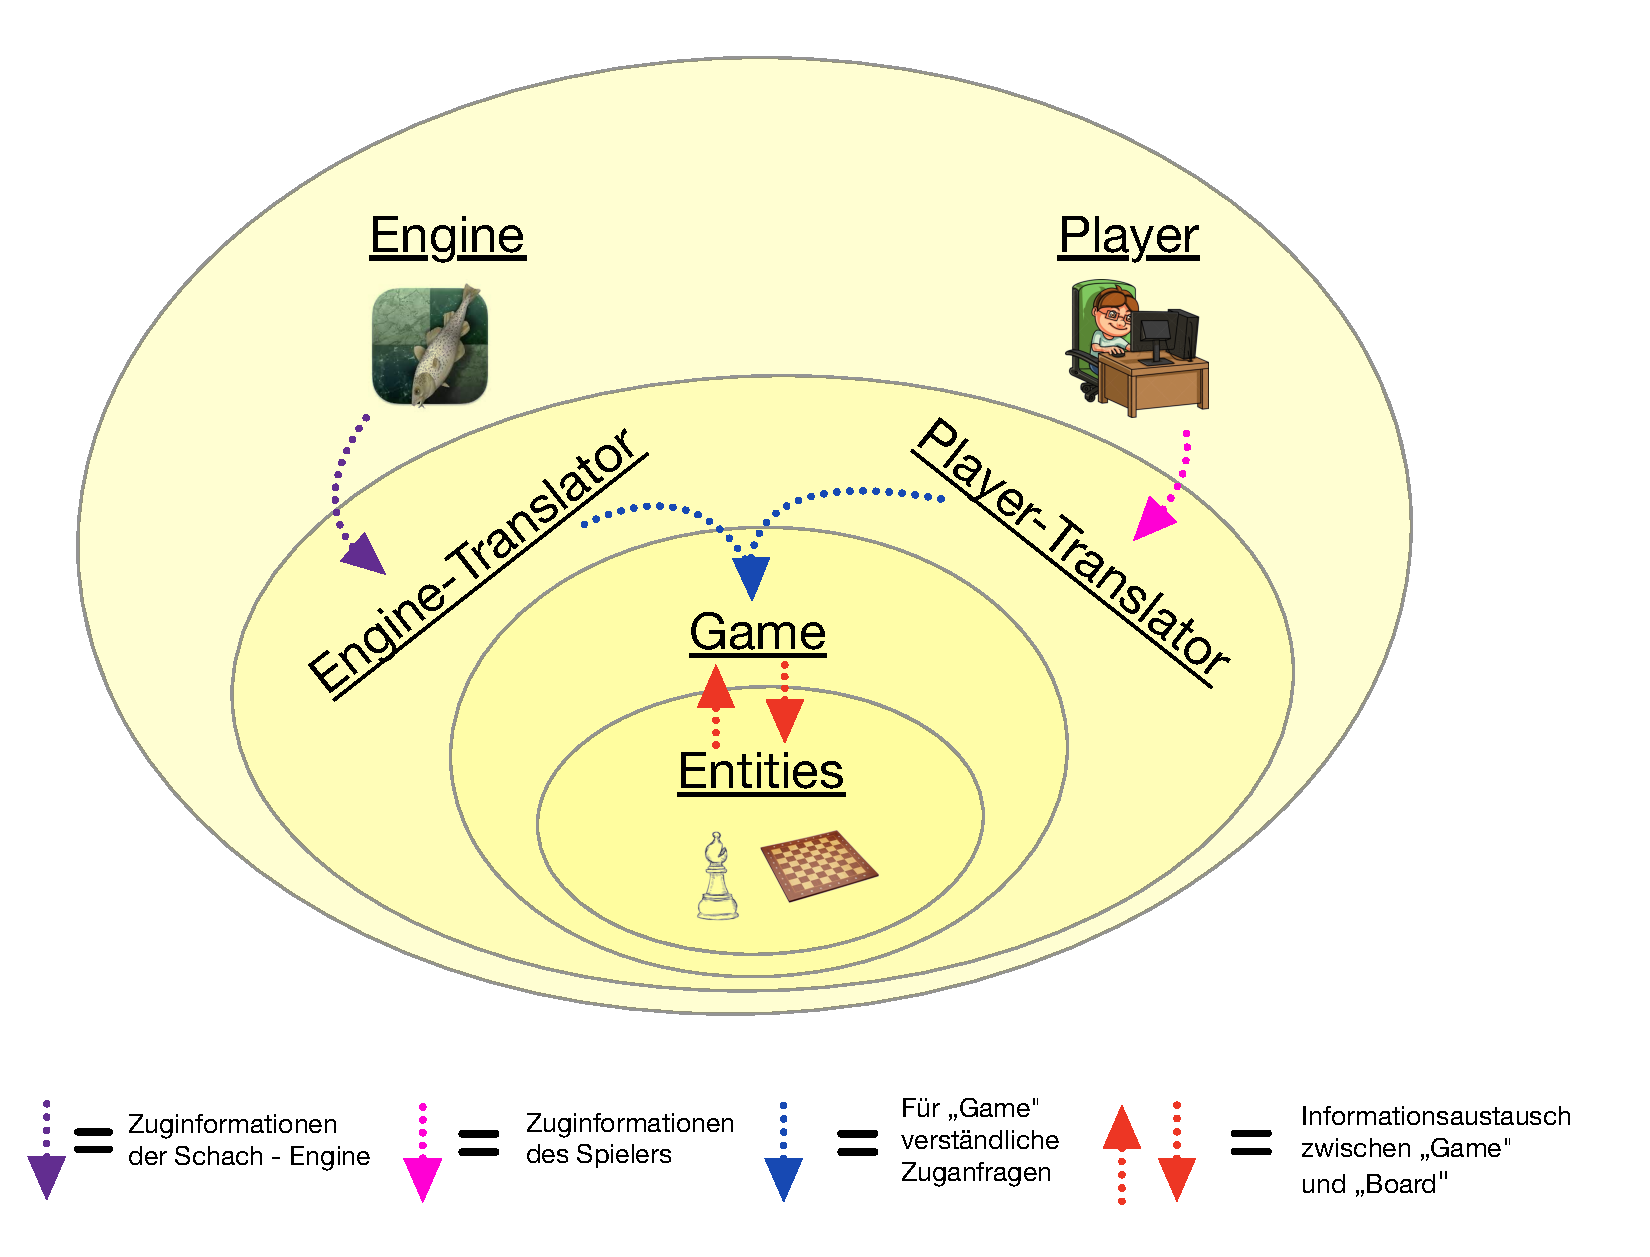
\includegraphics[width = \textwidth]{onion.pdf}
		\caption{Übersicht über unsere Form der Clean-Architecture}
		\label{pic:cleanArc}
	\end{center}
\end{figure}


Zusammengefasst ermöglicht eine Clean-Architecture die Veränderung der Umgebung, bzw. des Systems, ohne den eigentlichen Kern des Codes anpassen zu müssen.
Das bedeutet, dass wir theoretisch unser Spiel um ein echtes Spielbrett mit LED's und Arduino- oder Raspberry-Steuerung erweitern könnten, ohne den eigentlichen Schach-Code zu verändern.

\autoref{pic:cleanArc} zeigt eine grafische Übersicht über unsere Realisierung einer Clean-Architecture. Im Folgenden werden die hier zu sehenden einzelnen Schichten detailiert erklärt.

\newpage
\subsection{Schicht 1: Entities}
Die Entities bilden Kern unseres Spiels. Unabhängig von der Umgebung sind die einzelnen Figuren virtuell auf einem Feld positioniert und können umplatziert werden.
Folgende Klassen ergeben sich aus diesem Konzept: 

\begin{center}
	\begin{itemize}
		\item \texttt{\href{https://github.com/schmida736/Chess-AdvancedSE/blob/main/Chess-AdvancedSE/Game\%20Elements/Board.cs}{Board}}
		\item \texttt{\href{https://github.com/schmida736/Chess-AdvancedSE/blob/main/Chess-AdvancedSE/Game\%20Elements/Square.cs}{Square}}
		\item \texttt{\href{https://github.com/schmida736/Chess-AdvancedSE/blob/main/Chess-AdvancedSE/Game\%20Elements/Pieces/Piece.cs}{Piece}}
	\end{itemize}
\end{center}

\texttt{\href{https://github.com/schmida736/Chess-AdvancedSE/blob/main/Chess-AdvancedSE/Game\%20Elements/Board.cs}{Board}} besteht aus mehreren \texttt{Squares}, auf denen jeweils ein \texttt{\href{https://github.com/schmida736/Chess-AdvancedSE/blob/main/Chess-AdvancedSE/Game\%20Elements/Pieces/Piece.cs}{Piece}} stehen kann. \autoref{pic:umlEntities} zeigt alle Klassen welche unser Kern der Clean-Architektur beinhalten soll. 
\vspace{0.4cm}
\begin{figure}[h]
	\begin{center}
		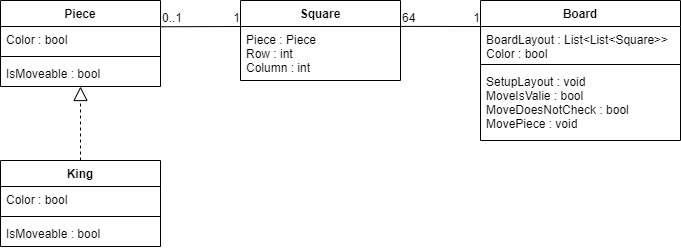
\includegraphics[width=13cm]{entities.png}
		\caption{\label{pic:umlEntities} UML-Diagramm der Entities}
	\end{center}
\end{figure}

Ein Schachbrett setzt sich aus 64 Feldern zusammen. Die Methode \texttt{SetupLayout} erstellt das Spielbrett (\texttt{\href{https://github.com/schmida736/Chess-AdvancedSE/blob/main/Chess-AdvancedSE/Game\%20Elements/Board.cs}{Board}}) und besetzt einige der Felder (\texttt{\href{https://github.com/schmida736/Chess-AdvancedSE/blob/main/Chess-AdvancedSE/Game\%20Elements/Square.cs}{Square}}) mit Figuren (\texttt{\href{https://github.com/schmida736/Chess-AdvancedSE/blob/main/Chess-AdvancedSE/Game\%20Elements/Pieces/Piece.cs}{Piece}}) einer entsprechenden Farbe.
In \autoref{pic:umlEntities} steht der König (\texttt{\href{https://github.com/schmida736/Chess-AdvancedSE/blob/main/Chess-AdvancedSE/Game\%20Elements/Pieces/King.cs}{King}}) für alle Figuren. Die anderen implementieren, genau wie er, die Methode \texttt{IsMoveable}.
\texttt{\href{https://github.com/schmida736/Chess-AdvancedSE/blob/main/Chess-AdvancedSE/Game\%20Elements/Board.cs}{Board}} bietet drei Methoden, wobei nur \texttt{MovePiece} von weiteren Schichten verwendet wird. Diese Methode überprüft mit \texttt{MoveIsValid}, ob es sich um einen validen Zug handelt. \texttt{MoveIsValid} ruft dabei die von Figuren implementierte Methode \texttt{IsMoveable} auf um zu überprüfen ob die Figur theoretisch in der Lage wäre den Zug durchzuführen.\\ 
Der wesentliche Unterschied zwischen \texttt{MoveIsValid} und \texttt{IsMoveable} besteht darin, dass Figuren das \href{https://github.com/schmida736/Chess-AdvancedSE/blob/main/Chess-AdvancedSE/Game\%20Elements/Board.cs}{Board} nicht kennen und auch nicht wissen wo sie sich befinden. \texttt{IsMoveable} signalisiert lediglich, ob ein Zug rein von den allgemeinen Zugmöglichkeiten der Figur möglich ist (z.B. Läufer kann nur schräg laufen). \texttt{MoveIsValid} ist eine Methode des Boards und kann somit auch situationsbedingte Auskunft über die Validität des Zuges geben. Ist die Figur \texttt{IsMoveable}, wird von \texttt{MoveIsValid} noch überprüft ob weitere Figuren im Weg stehen und der Zug sich selbst in Schach setzen würde (\texttt{MoveDoesNotCheck}). Ist alles überprüft, wird der Zug durchgeführt.

\subsection{Schicht 2: Use-Case}
Use-Cases bilden die zweite Schicht der Clean Architekture. Sie können Informationen der ersten Schicht (Entities) erhalten.\\
Wir haben nur einen Use-Case: Das Spiel, bzw. \texttt{\href{https://github.com/schmida736/Chess-AdvancedSE/blob/main/Chess-AdvancedSE/Game\%20Elements/Game.cs}{Game}} . Diese Klasse erstellt ein \texttt{\href{https://github.com/schmida736/Chess-AdvancedSE/blob/main/Chess-AdvancedSE/Game\%20Elements/Board.cs}{Board}}, bzw ruft die Funktion \texttt{SetupLayout} auf. Sie besitzt aber noch weitere Informationen die über das einfache Ziehen von Figuren hinausgehen:
\begin{center}
	\begin{itemize}
		\item Spielerposition (z.B. Spieler 1 spielt unten),
		\item Spielerfarbe (z.B. Spieler 1 ist weiß)
		\item und aktueller Spieler (z.B. Spieler 1 ist dran).
	\end{itemize}
\end{center}
Beim Erstellen von \texttt{\href{https://github.com/schmida736/Chess-AdvancedSE/blob/main/Chess-AdvancedSE/Game\%20Elements/Board.cs}{Board}} wird die Farbe des unten spielenden Spielers zufällig gewählt. Logisch betrachtet spielt für \texttt{\href{https://github.com/schmida736/Chess-AdvancedSE/blob/main/Chess-AdvancedSE/Game\%20Elements/Game.cs}{Game}} Spieler 1 in jedem Fall \textit{unten}. Da immer weiß beginnt, ist es zufällig, ob Spieler 1 beginnen darf, oder nicht. Welche Art von User-Interface nun Spieler 1 steuert, ist Aufgabe der dritten Schicht, welche in unserem Fall den Menschen, spielend übe die Benutzeroberfläche, Spieler 1 und eine Schach-Engine Spieler 2 zuordnet. \texttt{\href{https://github.com/schmida736/Chess-AdvancedSE/blob/main/Chess-AdvancedSE/Game\%20Elements/Game.cs}{Game}} ist von dieser Information jedoch abgekapselt, da eine Zuganfrage in jedem Fall gleich codiert ist.
\texttt{\href{https://github.com/schmida736/Chess-AdvancedSE/blob/main/Chess-AdvancedSE/Game\%20Elements/Game.cs}{Game}} soll die Anfragen als String (z.B. 'e5,e6' = ''Zug von e5 nach e6'') definieren. \\
Wird nun eine solche Anfrage gestellt, verlangt \texttt{\href{https://github.com/schmida736/Chess-AdvancedSE/blob/main/Chess-AdvancedSE/Game\%20Elements/Game.cs}{Game}} von \texttt{\href{https://github.com/schmida736/Chess-AdvancedSE/blob/main/Chess-AdvancedSE/Game\%20Elements/Board.cs}{Board}} eine Auskunft über die Farbe der Figur, welche sich auf dem \textit{von}-Feld befindet. Stimmt diese mit der Farbe des aktuell spielenden Spielers überein, kann der Zug nach Validitätsprüfung ausgeführt werden. Anhand dessen ob \texttt{MovePiece} \texttt{true} oder \texttt{false} zurückgibt, ist der andere Spieler daraufhin am Zug, oder nicht.
\subsection{Schicht 3: Übersetzer}
Sollte es dazu kommen, dass die Umgebung beispielsweise gegen eine Ascii-Oberfläche ausgetauscht wird, müssen ab dieser Schicht Veränderungen am Code erfolgen. Solange jedoch die Zug-Anfragen richtig gestellt werden, arbeitet der Code in den unteren Schichten immer gleich. In der dritten Schicht befindet sich ein GUI- und Engine-Translator. Diese übersetzen Züge von Benutzeroberfläche / Engine und geben sie codiert an die zweite Schicht. Zwischen den Translatorn und \texttt{\href{https://github.com/schmida736/Chess-AdvancedSE/blob/main/Chess-AdvancedSE/Game\%20Elements/Game.cs}{Game}} findet sich eine Dependency Inversion. Mehr dazu unter \autoref{sec:depin}
Solche Zug-Anfragen können völlig asynchron erfolgen. Sie führen jedoch zu nichts, falls der Zug nicht regelkomform, oder der Spielende nicht am Zug ist.
\subsection{Schicht 4: User-Interfaces}
Auf dieser Ebene befinden sich Interfaces für die Spieler. In unserem Fall sind das Benutzeroberfläche und Schachengine. Die Oberfläche wurde mit WPF gebaut. Dieses stellt mithilfe eines Databindigs auf ein Viewmodel von \texttt{\href{https://github.com/schmida736/Chess-AdvancedSE/blob/main/Chess-AdvancedSE/Game\%20Elements/Board.cs}{Board}-Layouts} immer den aktuellen Stand des Spiels grafisch dar. 
Dabei ist die Möglichkeit geboten, mithilfe von Mausklicks Figuren zu ziehen (z.B. erster Klick auf \textit{E2}, zweiter Klick auf \textit{E3}~~ $\Rightarrow$ \textit{E2 nach E3}). Diese Klicks werden dann an \texttt{PlayerTranslator} in der dritten Schicht weitergegeben, welcher diese dann in eine für \texttt{\href{https://github.com/schmida736/Chess-AdvancedSE/blob/main/Chess-AdvancedSE/Game\%20Elements/Game.cs}{Game}} verständliche Anweisungen übersetzt.
Da unter WPF das Main-Window als erstes erstellt wird, befindet sich hier auch unsere Main. Sie erstellt auch das \href{https://github.com/schmida736/Chess-AdvancedSE/blob/main/Chess-AdvancedSE/Game\%20Elements/Game.cs}{Game}, wodurch die ganze Schachlogik gestartet wird.

Die Einbindung der Engine funktioniert ähnlich, nämlich über \texttt{EngineTranslator}, welcher als Schnittstelle zwischen \texttt{\href{https://github.com/schmida736/Chess-AdvancedSE/blob/main/Chess-AdvancedSE/Game\%20Elements/Game.cs}{Game}} und Engine dient. Der größte Unterschied ist hier, dass die Engine als eine externe Kommandozeilenanwendung realisiert ist und daher erst einmal in unsere C\#-Anwendung eingebunden werden muss.
Hierfür wird eine Instanz einer Engine-Klasse erstellt, welche den tatsächlichen Engine-Pozess startet und sich um sämtliche Kommunikation zwischen dem Engine-Prozess und dem \texttt{EngineTranslator} kümmert. Vom EngineTranslator wird hier regelmäßig das aktuelle Layout des Boards abgefragt. Dieses wird dann an die Engine weitergeleitet, welche daraufhin den nächsten besten Zug berechnet. Dieser berechnete Zug wird dann an den Translator zurückgegeben, welcher diesen dann übersetzt und an das Spiel weitergibt.
\newpage
\section{Programmierprinzipien}
Programmierprinzipien sind allgemeine, kontextunabhängige Regeln, die als Grundlage für das Vorgehen in oft wiederkehrenden Situationen während der Programmierung dienen sollen.\\
In diesem Kaptitel betrachten wir einige Prinzipien und zeigen, wie wir sie in unserem Projekt umgesetzt haben.
\subsection{Single Resposibility Principle}
Das Single Resposibility Principle(SRP) besagt, dass eine Klasse immer nur einen Grund zur Veränderung haben darf. Dies bedeutet, dass jede Klasse sich auf eine klar abgegrenzte Tätigkeit beschränken sollte. 
\\
Durch Befolgung des SRP soll verhindert werden, dass riesige \enquote{alleskönner}-Klassen entstehen, die bei jeder Veränderung (z.B der externen Abhängigkeiten) komplett überarbeitet werden müssen. Schlimmer noch kann bei Nichtbefolgung passieren, dass sich unbemerkt Zuständigkeitsüberlappungen zwischen mehreren Klassen bilden. Bei Veränderung müssen dann nicht nur eine Klasse sondern gleich mehrere überarbeitet werden.
\\
Ein Beispiel für die Einhaltung des SRP in unserem Projekt findet sich in unserer Aufteilung von \href{https://github.com/schmida736/Chess-AdvancedSE/blob/main/Chess-AdvancedSE/Game\%20Elements/Board.cs}{Board} und \href{https://github.com/schmida736/Chess-AdvancedSE/blob/main/Chess-AdvancedSE/Game\%20Elements/BoardLayout.cs}{BoardLayout}. Hier übernimmt die Klasse \texttt{\href{https://github.com/schmida736/Chess-AdvancedSE/blob/main/Chess-AdvancedSE/Game\%20Elements/Board.cs}{Board}} sämtliche Aufgaben, die mit Zugbefehlen und der Koordinierung der Schachfiguren zu tun haben. \href{https://github.com/schmida736/Chess-AdvancedSE/blob/main/Chess-AdvancedSE/Game\%20Elements/BoardLayout.cs}{BoardLayout} hingegen speichert und beeinflusst die Aufstellung des Schachbretts.
\\
\href{https://github.com/schmida736/Chess-AdvancedSE/blob/main/Chess-AdvancedSE/Game\%20Elements/BoardLayout.cs}{BoardLayout} war ursprünglich Teil der \href{https://github.com/schmida736/Chess-AdvancedSE/blob/main/Chess-AdvancedSE/Game\%20Elements/Board.cs}{Board}-Klasse, doch als die Klasse begann immer größer zu werden und immer mehr Funktionalität in sich zu vereinen, beschlossen wir sie in zwei Klassen aufzuteilen.
\texttt{\href{https://github.com/schmida736/Chess-AdvancedSE/blob/main/Chess-AdvancedSE/Game\%20Elements/Board.cs}{Board}} nutzt nun die Methoden von \texttt{\href{https://github.com/schmida736/Chess-AdvancedSE/blob/main/Chess-AdvancedSE/Game\%20Elements/BoardLayout.cs}{BoardLayout}}, um Einfluss auf die Aufstellung des Schachbretts zu nehmen.
\\
Diese Änderung ermöglicht es uns, die Schachbrett-Logik separat von der Zug und Figuren-Logik zu testen. Das vereinfacht das Erstellen der Tests und das Finden der Fehlerquelle beim Fehlschlagen eines Tests.
\subsection{Open/Closed Principle}
Das Open/Closed Principle besagt, dass existierender Code wenn möglich
\begin{itemize}
	\item offen für Erweiterung
	\item geschlossen bezüglich Veränderung
\end{itemize}
sein sollte.
Das bedeutet, ein Modul sollte über klar definierte Schnittstellen einfach erweiterbar sein, jedoch an sonsten keine/sehr wenig Modifikation an bestehendem Code für eben solche Erweiterungen benötigen.
Ein Beispiel für dieses Prinzip an unserem Code wurde durch die Schichtarchitektur geschaffen. Über einen spezifischen \texttt{Translator} kann jede beliebige Schnittstelle hinzugefügt werden, um Züge an das \href{https://github.com/schmida736/Chess-AdvancedSE/blob/main/Chess-AdvancedSE/Game\%20Elements/Game.cs}{Game} zu schicken, es ist \textsl{offen bezüglich Erweiterung}. Das \href{https://github.com/schmida736/Chess-AdvancedSE/blob/main/Chess-AdvancedSE/Game\%20Elements/Game.cs}{Game} muss dafür nicht verändert werden, es ist \textsl{geschlossen bezüglich Veränderung}. So könnte zum Beispiel die Engine-Schnittstelle durch eine weiter GUI ersetzt werden, und so das Spiel für zwei Spieler spielbar werden. Hierfür müsste nur die Engine und der EngineTranslator entfernt werden, und ein spezifischer PlayerTranslator für die neue GUI geschrieben werden, der deren Züge in das für das \href{https://github.com/schmida736/Chess-AdvancedSE/blob/main/Chess-AdvancedSE/Game\%20Elements/Game.cs}{Game} verständliche Befehle umwandelt. Dieser kann dann die nötigen Methoden von \href{https://github.com/schmida736/Chess-AdvancedSE/blob/main/Chess-AdvancedSE/Game\%20Elements/Game.cs}{Game} aufrufen, ohne dass an diesem entwas verändert werden muss.
\subsection{Liskov' Substitution Principle}
Das Liskov Substitution Principle(LSP) besagt, dass jede Verwendung eines Objekts einer übergeordneten Klasse durch ein beliebiges Objekt einer ihrer Unterklassen ersetzbar sein soll. Durch das ersetzen darf sich die Korrektheit des Programms nicht ändern.

Dies setzt voraus, das jede Subklasse sich so verhält wie ihre Superklasse. Eine Subklasse darf also nicht die Funktionalität der Klasse einschränken, von der sie erbt, sie darf sie nur übernehmen und/oder erweitern. Das Ziel ist es, strenge Regeln für Vererbungshierarchien zu definieren und damit auf dem Varianzensystem der Vererbung aufzubauen. Bei konsequenter Befolgung des LSP kann vermieden werden, dass bei der Verwendung von Klassen falsche Annahmen aufgrund von Eigenschaften wie zum Beispiel dem Klassennahmen getroffen werden. Man kann bei code der dem LSP folgt nämlich stets davon ausgehen, dass Unterklassen immer alle Funktionalitäten der Oberklasse bereitstellt.
\\
Wir halten uns überall, wo wir in unserem Projekt Vererbung einsetzen, an das LSP. Unsere Figurenhierarchie basiert sogar darauf, dass wir die Funktion der allgemeinen Oberklasse \href{https://github.com/schmida736/Chess-AdvancedSE/blob/main/Chess-AdvancedSE/Game\%20Elements/Pieces/Piece.cs}{Piece} in ihren Unterklassen erweitern. Wir benutzen \href{https://github.com/schmida736/Chess-AdvancedSE/blob/main/Chess-AdvancedSE/Game\%20Elements/Pieces/Piece.cs}{Piece} oft als eine verallgemeinerung der verschiedenen Figuren und durch polymorphe Aufrufe zur Laufzeit werden dann die Methoden der konkreten Figuren aufgerufen. \autoref{fig:be2bb473-a08a-4816-9d19-355c2e271155} ist ein Beispiel, in dem ein als \href{https://github.com/schmida736/Chess-AdvancedSE/blob/main/Chess-AdvancedSE/Game\%20Elements/Pieces/Piece.cs}{Piece} deklariertes Objekt zur Laufzeit eine Instanz einer ihrer Unterklassen zugewiesen wird und anschließend durch Laufzeitpolymorphie eine Methode dieser unterklasse ausgeführt wird.

\begin{figure}[ht]
	\centering
	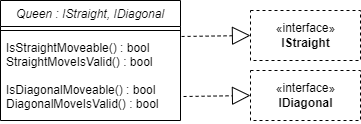
\includegraphics[width=0.5\linewidth]{Diagonal_Straight.png}
	\caption[Interface Segregation auf Queen]{Interface Segregation auf Queen}
	\label{fig:int_seg}
\end{figure}

\subsection{Interface Segregation Principle}
Schon bei Beginn des Projekts war geplant, Interfaces für die Züge einzelner Figuren einzusetzen. Da jede Figur zur Zugvalidierung die Methoden \texttt{IsMoveable} und \texttt{MoveIsValid} besitzt, wäre hierfür ein Interface, welches diese Methoden vordefiniert die richtige Wahl. Der erste Gedanke war ein Interface namens \texttt{IMoveable}, welches die oben genannten Methoden definiert. Jede Figur könnte so beide Methoden individuell implementieren. Dabei wäre aber das Interface Segregation Principle verletzt, da das Interface somit für alle möglichen Zugarten zuständig wäre. Eine Figur die schräg zieht, implementierte somit die gleichen Methoden wie ein Geradezieher. Daher haben wir das Interface in \texttt{\href{https://github.com/schmida736/Chess-AdvancedSE/blob/main/Chess-AdvancedSE/Game\%20Elements/Pieces/IStraight.cs}{IStraight}} für gerade und \texttt{\href{https://github.com/schmida736/Chess-AdvancedSE/blob/main/Chess-AdvancedSE/Game\%20Elements/Pieces/IDiagonal.cs}{IDiagonal}} für schräge Züge aufgeteilt. In \autoref{pic:MoveInterfaces} ist diese aufteilung zu sehen. Ein König würde ebenfalls sowohl \texttt{\href{https://github.com/schmida736/Chess-AdvancedSE/blob/main/Chess-AdvancedSE/Game\%20Elements/Pieces/IStraight.cs}{IStraight}}, als auch \texttt{\href{https://github.com/schmida736/Chess-AdvancedSE/blob/main/Chess-AdvancedSE/Game\%20Elements/Pieces/IDiagonal.cs}{IDiagonal}} implementieren. In seinem Fall jedoch im Gegensatz zur Dame nur mit einer maximalen Zuglänge von $1$.

\subsection{Dependency Inversion Principle}
\label{sec:depin}
Das Dependency Inversion Principle(DIP) ist das letzte der 5 SOLID-Prinzipien. Es ist das Prinzip der Entkopplung und besagt, dass Abstaktionen nicht von Details abhängen sollten, sondern umgekehrt. Daraus folgt für eine Software-Architektur, die den SOLID-Prinzipien folgt, dass ihre Module hoher Ebenen nicht abhängig von Modulen niedriger Ebenen sein sollen.
Wir haben das DIP in der verbindung zwischen \href{https://github.com/schmida736/Chess-AdvancedSE/blob/main/Chess-AdvancedSE/Game\%20Elements/Game.cs}{Game} und den Translators angwendet, da die sie sich in einer höheren Ebene befinden als \href{https://github.com/schmida736/Chess-AdvancedSE/blob/main/Chess-AdvancedSE/Game\%20Elements/Game.cs}{Game}, aber mit ihm kommunizieren können müssen.
Um zu vermeiden, eine direkte Referenz auf \href{https://github.com/schmida736/Chess-AdvancedSE/blob/main/Chess-AdvancedSE/Game\%20Elements/Game.cs}{Game} Beispielsweise in PlayerTranslator verwenden zu müssen und damit von der konkreten Umsetzung von \href{https://github.com/schmida736/Chess-AdvancedSE/blob/main/Chess-AdvancedSE/Game\%20Elements/Game.cs}{Game} abhängig zu sein, haben wir die für den Translator wichtigen Schnittstellen in ein IGame Interface ausgelagert. PlayerTranslator agiert nun auf diesen Schnittstellen, kennt aber nicht die genaue Implementierung von \href{https://github.com/schmida736/Chess-AdvancedSE/blob/main/Chess-AdvancedSE/Game\%20Elements/Game.cs}{Game} und ist daher nicht darauf angewiesen, dass diese unverändert bleiben.
\subsection{Low Coupling}
Low Coupling ist ein GRASP-Prinzip der Objektorientierten Softwarearchitektur, nach dem eine Klasse so unabhängig von ihrer Umgebung sein sollte wie möglich. Dies macht es einfacher, die Funtionsweise der Klasse nachzuvollziehen, weil man weniger Klassen verstehen muss, von denen diese eine Klasse abhängig ist. Des weiteren erzielt eine lose Kopplung einer Klasse auch eine deutlich höhere Testbarkeit, da weniger instanzen von abhängigen Klassen erstellt werden müssen, nur um eine Klasse zu testen(siehe Negativbeispiel).

\subsubsection{Beispiel}
Durch unsere Clean Architecture haben wir eine Architektur aufgebaut, die es den einzelnen Schichten erlaubt, unabhängig von den Elementen der über ihnen liegenden Schichten zu sein. So ist auf \autoref{pic:cleanArc} zu sehen, dass \href{https://github.com/schmida736/Chess-AdvancedSE/blob/main/Chess-AdvancedSE/Game\%20Elements/Game.cs}{Game} komplett unabhängig von PlayerTranslator und EngineTranslator ist. Es erhät ausschließlich Anweisungen per Methodenaufruf und führt diese aus. \href{https://github.com/schmida736/Chess-AdvancedSE/blob/main/Chess-AdvancedSE/Game\%20Elements/Game.cs}{Game} weiß nicht, dass es eine GUI oder eine Engine gibt, es interessiert sich nur an den von oben kommenden Befehlen. Dies bedeutet, dass \href{https://github.com/schmida736/Chess-AdvancedSE/blob/main/Chess-AdvancedSE/Game\%20Elements/Game.cs}{Game} abgekoppelt von sowohl den User-Interfaces, als auch von den Übersetzern ist.

\subsubsection{Negativbeispiel}
Ein Neagtivbeispiel für Low Coupling sind bei unserer Architektur die Kopplung zwischen der Klasse \href{https://github.com/schmida736/Chess-AdvancedSE/blob/main/Chess-AdvancedSE/Game\%20Elements/Board.cs}{Board} und den Pieces. Diese müssen miteinander kommunizieren können, und brauchen daher jeweils Referenzen aufeinander. Dies führt dazu, dass die Testbarkeit von Pieces erheblich reduziert ist. Sichtbar wird dies in den Unit Tests der Pieces (TestPieces.cs). Da jedes \href{https://github.com/schmida736/Chess-AdvancedSE/blob/main/Chess-AdvancedSE/Game\%20Elements/Pieces/Piece.cs}{Piece} eine Referenz auf das in \href{https://github.com/schmida736/Chess-AdvancedSE/blob/main/Chess-AdvancedSE/Game\%20Elements/Board.cs}{Board} enthaltene \href{https://github.com/schmida736/Chess-AdvancedSE/blob/main/Chess-AdvancedSE/Game\%20Elements/BoardLayout.cs}{BoardLayout} braucht, muss ein solches Layout in jedem Unit Test so erzeugt werden, wie der Test es gerade braucht.

\subsection{High Cohesion}
Kohäsion ist ein Maß für den inneren Zusammenhalt einer Klasse. Hierbei möchten wir Ihnen zeigen, dass wir das Prinzip verstanden haben, indem wir ein Positiv- und Negativbeispiel darstellen. Beide dieser Beispiele befinden sich in der Klasse \texttt{\href{https://github.com/schmida736/Chess-AdvancedSE/blob/main/Chess-AdvancedSE/Game\%20Elements/Pieces/Bishop.cs}{Bishop}}. Die Klasse, mit farblichen Markierungen zur besseren Kohäsionsdarstellung, ist in \autoref{pic:koh} gezeigt.

\begin{figure}[h]
	\begin{center}
		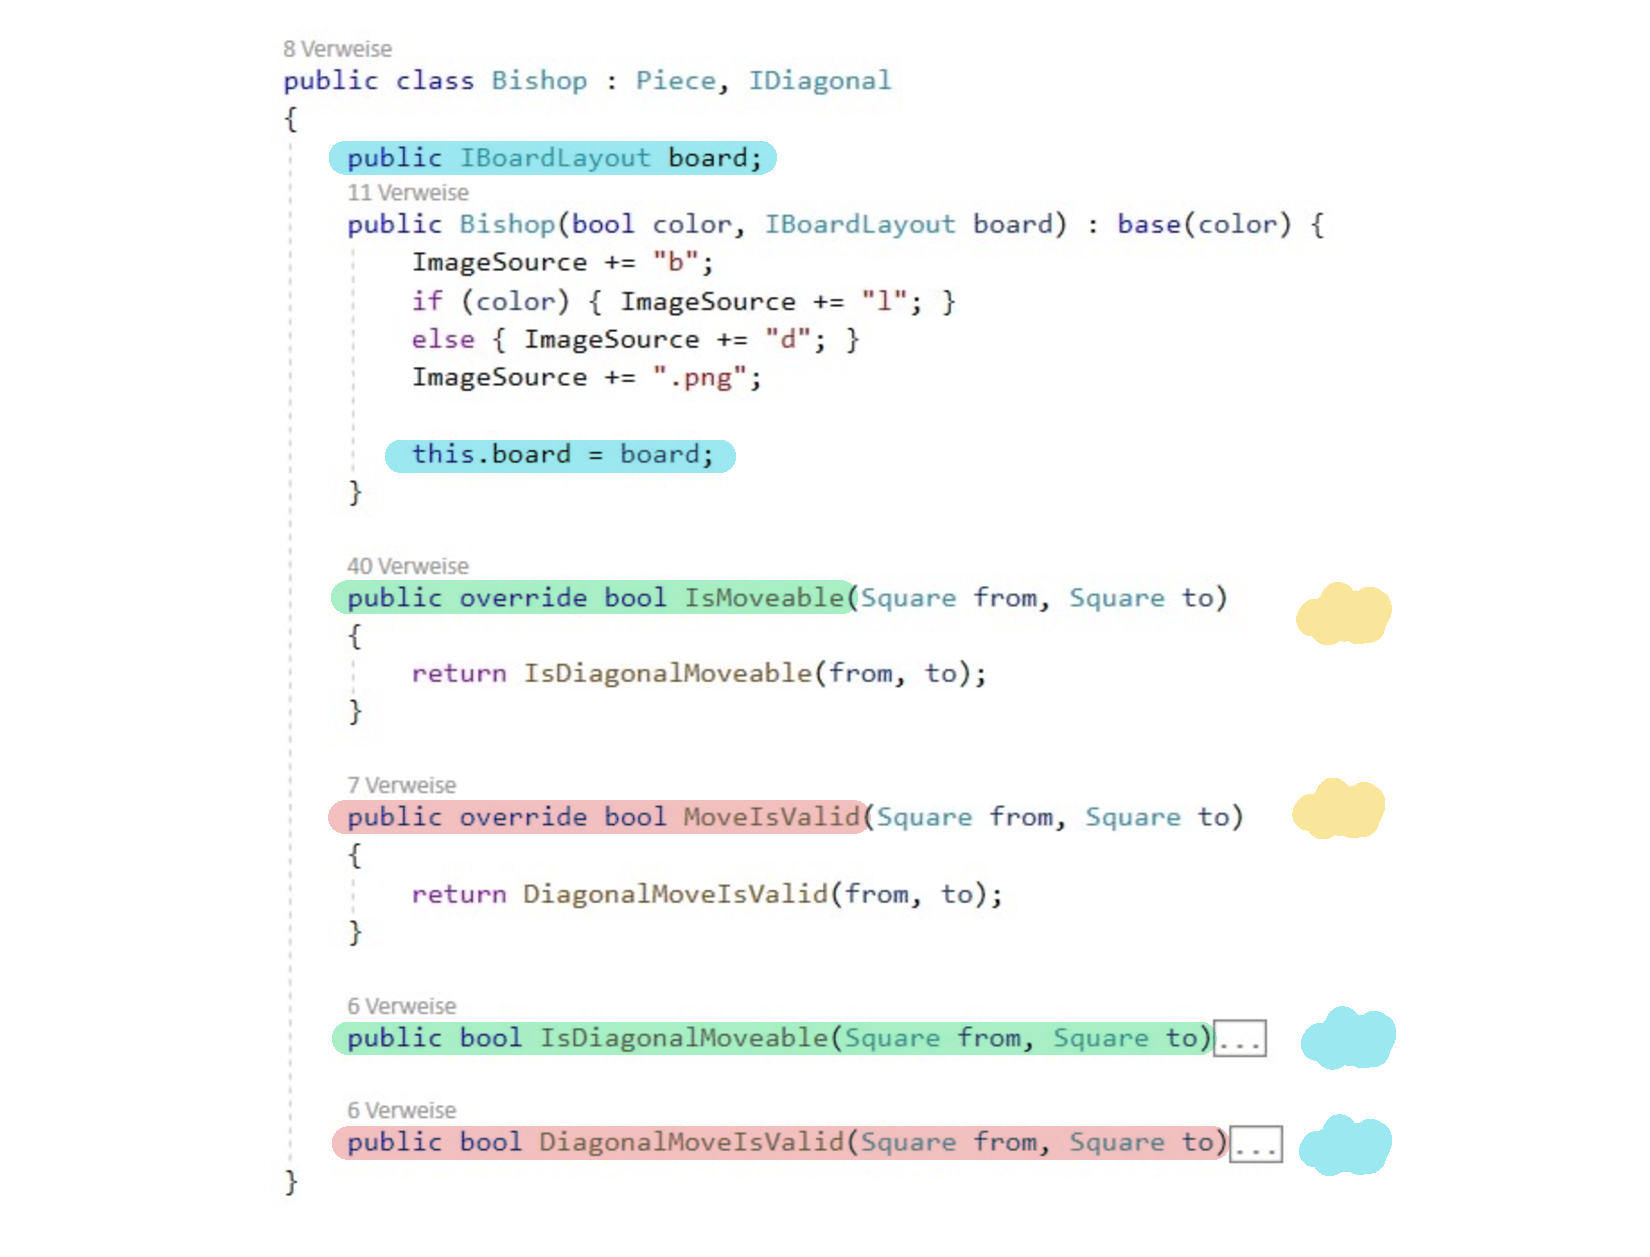
\includegraphics[width=\textwidth]{Kohaesion.pdf}
		\caption{\label{pic:koh} Kohäsionsbeispiel anhand von \texttt{\href{https://github.com/schmida736/Chess-AdvancedSE/blob/main/Chess-AdvancedSE/Game\%20Elements/Pieces/Bishop.cs}{Bishop}}}
	\end{center}
\end{figure}

Blau markiert sind in diesem Beispiel Deklaration und Einsatz von \texttt{board}. Es wird verwendet, um Züge zu validieren. Daher kommen auch die blauen Kringel neben den Methoden, wo die Variable verwendet wird. Die jeweils rot und grün markierten Methoden arbeiten zusammen. Innerhalb der Klasse sind sie zwar syntaktisch nicht verbunden, sie dienen aber semantisch dem gleichen Zweck. Dies ist in \autoref{pic:koh} durch den gelben Kringel verdeutlicht. Eine Methode welche \texttt{IsMoveable $\&\&$ MoveIsValid} als bool zurückgibt, gäbe eine fast vollständige Zugvalidierung zurück. Da jedoch noch andere Sachen wie beispielsweise das in Schachsetzen dabei eine Rolle spielen, ist dieser Zusammenhalt in der Klasse \texttt{\href{https://github.com/schmida736/Chess-AdvancedSE/blob/main/Chess-AdvancedSE/Game\%20Elements/Board.cs}{Board}} und nicht hier aufgeführt. 
Negativ zu bemerken sind die nicht-markierten Zeilen im Konstruktor der Klasse. Hierbei wird eine Bildquelle festgelegt, die jedoch mit dem Rest der Klasse nichts zu tun hat. Wäre dies abgekapselt, würde die Klasse eine extrem hohe Kohäsion nachweisen können.




\subsection{DRY (Don't Repeat Yourself)}
Im Folgenden sind auch bei diesem Prinzip sowohl ein Positiv- als auch ein Negativbeispiel für DRY aufgezeigt. 

\subsubsection{Negativbeispiel}
Eine Übersicht über die hier zur Darstellung verwendeten Klassen und Interfaces ist in \autoref{pic:MoveInterfaces} gezeigt.

\begin{figure}[h]
	\begin{center}
		\includegraphics[width=11cm]{MoveInterfaces.png}
		\caption{\label{pic:MoveInterfaces}Klassen und Interfaces für schräges und gerades Ziehen}
	\end{center}
\end{figure}

Dame, Läufer und Turm sind in ihrem Handlungsspielraum recht ähnlich. Ein Läufer kann nur schräg, ein Turm nur geradeaus ziehen. Eine Dame beherrscht beide dieser Zugarten. In unserem Code haben wir ein Interface für sowohl gerade, als auch schräge Züge. Die oben genannten drei Figuren implementieren jeweils die zugspezifischen Methoden für \texttt{IsMoveable} und \texttt{MoveIsValid}. 
Eine Implementierung der Methode \texttt{StraightMoveIsValid} des Turms findet sich $1:1$ bei der Dame wieder. \texttt{\href{https://github.com/schmida736/Chess-AdvancedSE/blob/main/Chess-AdvancedSE/Game\%20Elements/Pieces/Queen.cs}{Queen}} kopiert zudem auch die Methoden zur schrägen Zugvalidierung welche auch im Läufer zu finden sind. Dadurch sind die Methoden für schräges und gerades Laufen doppelt ohne Unterschied implementiert. Eine komplexere Klassenhierarchie für die einzelnen Figuren hätte hier Abhilfe schaffen können. Dadurch wären die besagten Methoden an einem zentralen Punkt vorgegeben und werden von einzelnen Figuren nur geerbt, ohne dass sie hier doppelt zu implementieren sind.

\subsubsection{Positivbeispiel}
Die unter \autoref{sec:replTemp} genutzte Methode \texttt{GetSquareDistance} wird von fast jeder Figur verwendet. Anstatt diese jeweils innerhalb einer Figurenklasse wie \texttt{\href{https://github.com/schmida736/Chess-AdvancedSE/blob/main/Chess-AdvancedSE/Game\%20Elements/Pieces/Queen.cs}{Queen}} zu platzieren, wird die Methode von \texttt{\href{https://github.com/schmida736/Chess-AdvancedSE/blob/main/Chess-AdvancedSE/Game\%20Elements/Pieces/Piece.cs}{Piece}} implementiert. Da alle Figuren von \texttt{\href{https://github.com/schmida736/Chess-AdvancedSE/blob/main/Chess-AdvancedSE/Game\%20Elements/Pieces/Piece.cs}{Piece}} erben, können sie auf die Methode zugreifen, welche jedoch so nur ein einziges Mal im Code ausprogrammiert ist. Dadurch ist, wenn auch nur anhand einer simplem Methode, \textit{DRY} richtig dargestellt.
\newpage
\section{Unit Testing}
\subsection{pros/cons/wieso wir?}
Tests sind eine der grundlegenden Elemente einer jeder Software-Anwendung. Ohne sie kann der korrekte Ablauf der Anwendung nicht \dots getestet werden. Unit tests verwenden wir in unserem Projekt hauptsächlich dort, wo Berechnungen auf dem Brett durgeführt werden. Diese sind nämlich erfahrungsgemäß sehr fehleranfällig, besonders für die Art von Fehlern, die sich erst durch das Erweitern einer ursprünglichen Funktion einschleichen, entstehen hier sehr schnell. So ist es zum Beispiel gut möglich dass die Bewegungen des Bauerns perfekt regelkonform umgesetzt werden, jedoch nach der zusätzlichen Einführung der \enquote{En passant}-Schlagmöglichkeit plötzlich viele Züge wieder ausführbar sind, die gar nicht erlaubt sein sollten.

Für unser Projekt nutzen wir das C\# XUnit testing Framework, welches uns ermöglicht, ohne viel Aufwand Unit Tests zu erstellen.
XUnit tests sind nach dem folgenden Schema aufgebaut:
\begin{lstlisting}[language=c, style=mStyle]
public class TestClass{
	[Fact]
	public void TestUnit_NoDataPassed()
	{
		// Given
		bool b = false;

		// When
		b.Set(true);

		// Then
		Assert.True(b);
	}

	[Theory]
	[InlineData(1)]
	public void TestUnit_IntPassed(int input)
	{
		//Given
		int val;

		//When
		val = input;

		//Then
		Assert.Equal(1, val);
	}
}
\end{lstlisting}

Eine Testklasse wird verwendet, um zusammengehörende Unit Tests zu verpacken. Jeder Unit Test ist entweder mit \texttt{[Fact]} oder mit \texttt{Theory} annotiert. Das letztere wird verwendet, um zusätzliche externe Daten an den Test zu übergeben. Diese werden dann mit der \texttt{[InlineData]}-Annotation definiert und dann vor dem Test automatisch als Funktionsparameter übergeben.
\subsection{ATRIP}
Für das Entwickeln von guten Unit Tests gelten die ATRIP-Regeln, welche in den folgenden unterkapiteln aufgelistet werden.
\subsubsection{Automatic}
Gute Tests sollen automatisch, bedeutet ohne weiteres eingreifen des Entwicklers, ablaufen. Dazu gehört, dass die Tests regelmäßig automatisch gestartet werden und ihre Ergebnisse danach auch selbstständig überprüfen. Jeder Unit Test sollte nach Ablauf eines der beiden Ergebnisse \enquote{bestanden} und \enquote{nicht bestanden} zurückgeben.
An dieses Prinzip haben wir uns in sämtlichen Unit Test gehalten. Unsere Tests sind nach dem AAA(Arrange, Act, Assert)-Schema aufgebaut, bauen also zu Beginn die nötigen Abhängigkeiten auf, nehmen dann Einfluss auf diese und führen anschließend eine einzige Methode der xUnit.Assert-Klasse aus, um die Korrektheit des Endzustands zu prüfen. Unsere IDE Microsoft VisualStudio haben wir so konfiguriert, dass sämtliche Unit Tests jedes mal automatisch ausgeführt werden, nachdem der Build-Step des Projekts durchgelaufen ist.

\subsubsection{Thorough}
Tests sind \enquote{gründlich genug}, wenn jede missionskritische Eigenschaft getestet wird. Bei unserem Schachspiel sind solche missionskritischen Eigenschaften beispielsweise das korrekte und regelkomforme Verhalten der Figuren. 
\\
Des weiteren ist für gründliche Tests nötig, dass nach Auftreten eines Softwarefehlers ein Test geschrieben wird, der die Software auf genau diesen Fehler prüft. Damit kann man ein erneutes Auftreten des Fehlers vermeiden.
\\
Wie oben erwähnt ist das Testen des Verhaltens der Figuren sehr wichtig für unser Projekt. Dies hat vor allem zwei Gründe:
Zum einen würde ein Fehlverhalten der Figuren ein Schummeln der Spieler ermöglichen, und damit wahrscheinlich deren Spielspaß vermindern. 
Der zweite Grund ist, dass die Logik der Züge sehr komplex ist, es ist also sehr wahrscheinlich, dass sich hier Fehler ansammeln, die durch Tests gefunden werden können.
\\
Wir haben also besonders viel Wert auf das Testen der \href{https://github.com/schmida736/Chess-AdvancedSE/blob/main/Chess-AdvancedSE/Game\%20Elements/Pieces/Piece.cs}{Piece}-Familie gelegt, was daraus ersichtlich ist, dass 33 unserer 43 Unit Tests sich mit den verschiedenen Figuren beschäftigen.

Man kann allerdings bei unserm Testen noch nicht von \enquote{thorough} sprechen, denn die \href{https://github.com/schmida736/Chess-AdvancedSE/blob/main/Chess-AdvancedSE/Game\%20Elements/Board.cs}{Board}-Klasse ist auch sehr wichtig, konnte aber aus Zeitgründen nicht mehr vollständig mit Unit Tests abgedeckt werden.

\subsubsection{Repeatable}
Unit Tests sollten wiederholbar sein, was bedeutet, dass sie nicht auf veränderlichen Daten aufbauen sollten. Solche veränderlichen Daten sind beispielsweise Zufallszahlen, die aktuelle Uhrzeit oder die Anzahl von Dateien im Projektordner. Diese Art von Daten haben wir natürlich konsequent vermieden.
\subsubsection{Independent}
Die Kernaussage von independent Tests ist, dass die Ergebnisse oder die Funktion der Tests nicht abhängig von ihrer Reihenfolge oder Zusammenstellung sein dürfen. Jeder Test sollte vollständig unabhängig von allen anderen Tests sein. Dies haben wir erreicht, indem keine Ressource, die in einem Test verwendet wird, außerhalb dieses Tests weiterbesteht. Stattdessen wird jede Ressource, die ein Test benötigt in seiner Arrange-Phase erstellt und begrenzt sich damit auf den Scope des Tests.
\subsubsection{Professional}
Professionelle Unit Tests sind so einfach verständlich wie möglich gestaltet. Damit soll vermieden werden, das sich Fehler in den Test-Code einschleichen, da diese besonders schwierig und damit besonders teuer zu finden und beheben sind.
Unsere Unit Tests sind klein und überschaubar. Zudem ist unsere Namensgebung so gewählt, dass alle informationen über einen Test durch das Lesen seines Namens erhältlich sind. Ein Beispiel hierfür ist der folgende Unit Test:
\begin{lstlisting}[language=c, style=mStyle]
	[Fact]
	public void GetSquareFromCoords_ReturnedSquare_IsEmpty()
	{
		// Given
		BoardLayout layout = new();

		// When
		layout.SetToStartLayout(new Player());
		
		// Then
		Assert.Null(layout.GetSquareFromCoords(3, 3).Piece);
	}
\end{lstlisting}

\subsection{Code Coverage}
Code Coverage ist eine Metrik die angibt, wie 
groß der Anteil des von Tests abgedeckten Codes ist. Häufig genutze Varianten des Code Coverage sind Line Coverage und Branch Coverage.

Wir nutzen das Tool \texttt{Coverlet} für die generierung eines coverage-reports in XML-Format und das \texttt{ReportGenerator}-Tool für die generierung einer HTML-Übersicht der Ergebnisse.
\\
Diese Übersicht sieht dann folgendermaßen aus:
\begin{figure}[ht!]
	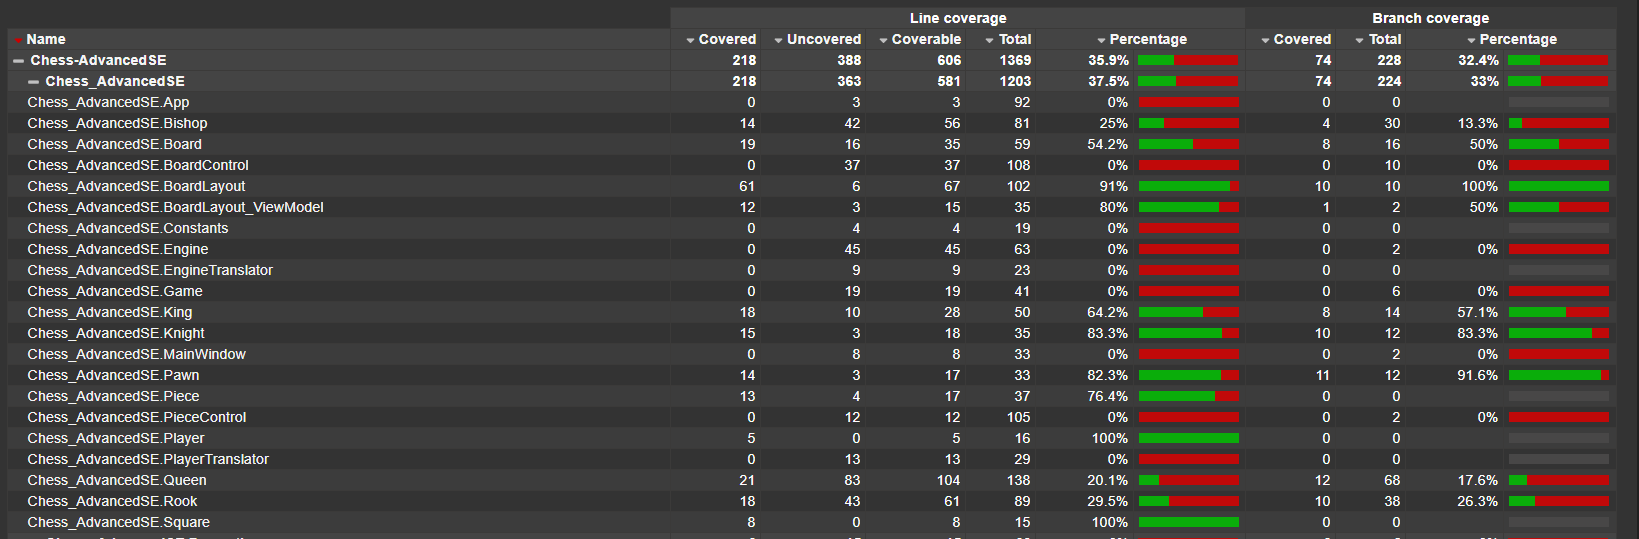
\includegraphics[width=\linewidth]{coveragereport}
\end{figure}

Sowohl Line Coverage als auch Branch Coverage sind hier aufgelistet. Unter den einzelnen Einträgen kann man sich dann die Details der Codeabdeckung ansehen.
Hier ein Beispiel:
\begin{figure}[ht!]
	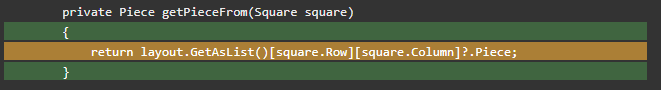
\includegraphics[width=\linewidth]{methodcovered}
\end{figure}

Wie man sieht, weist uns das Tool hier auf ein Problem hin: Hier ist nämlich eine lange Zeile mit mehreren Aufrufen, in der eine Abzweigung versteckt ist. Es wurde allerdings während unseren Unit Tests noch nicht überprüft, was passiert, wenn die Abzweigung ausgeführt wird, nämlich wenn das zurückgegebene \texttt{\href{https://github.com/schmida736/Chess-AdvancedSE/blob/main/Chess-AdvancedSE/Game\%20Elements/Square.cs}{Square}} \textsl{null} ist. Dies muss also in unseren Tests ergänzt werden.
\\
Die vollständige HTML-Übersicht kann über \href{https://github.com/schmida736/Chess-AdvancedSE/tree/main/Chess-AdvancedSE.Tests/coverage%20results}{diesen Link} eingesehen werden.

\newpage
\section{Refactoring}
\subsection{Codesmell: Long Method und Switch-case}
Einer früheren Version des Codes war eine Methode zu entnehmen, welche gleich zwei übel riechende Codesmells aufwies. Zum einen war die Methode sehr lang, zum anderen erstreckte sich ein großes Switch-Case über fast die gesamte Länge. Die Rede ist von jener Methode, welche festetellen soll, ob ein Zug valide ist, oder nicht. Zur Validierung muss ein Zug von einem Startfeld zu einem Zielfeld die folgenden Voraussetzungen erfüllen:
\begin{center}
	\begin{itemize}
		\item Das Zielfeld ist ein anderes als das Startfeld.
		\item Auf dem Startfeld steht eine Figur.
		\item Die Figur kann tatsächlich so ziehen.
		\item Der Zug würde das eigene Team nicht in Schach setzen.
		\item Der Zug darf so ausgeführt werden (d.h. es sind keine Figuren im Weg und am Ziel befindet sich keine Figur der eigenen Mannschaft).
	\end{itemize}
\end{center}
Ist eine dieser Anforderungen nicht erfüllt, wird der Zug als nicht valide gewertet. Wie bereits unter Clean-Architecture erwähnt, kann das \href{https://github.com/schmida736/Chess-AdvancedSE/blob/main/Chess-AdvancedSE/Game\%20Elements/Board.cs}{Board} situationsbedingte, die Figur hingegen nur über die theoretische Ausführung des Zuges Aussagen treffen. Dadurch ergab sich, dass die theoretische Ausführung eines Zuges polymorph innerhalb der Figuren und die situationsbedingte innerhalb von \texttt{MoveIsValid} evaluiert wurde. 
\vspace{0.5cm}

\begin{lstlisting}[language=c, style=mStyle]
public bool MoveIsValid(Square from, Square to)
{
 if (from.Row == to.Row && from.Column == to.Column) { return false; }
  if (layout.GetAsList()[from.Row][from.Column] != null)
  {
   Piece movingPiece = layout.GetAsList()[from.Row][from.Column].Piece;
   Piece destinationPiece = layout.GetAsList()[to.Row][to.Column].Piece;
   bool movingPieceColor = movingPiece.Color;
   if (movingPiece.IsMoveable(from, to) && MoveDoesNotCheck(from, to))
   {
	if (!movingPiece.MoveIsValid(from, to)) { return false; }
	switch (movingPiece)
	{
	 case Queen:
	  if (destinationPiece?.Color != movingPieceColor)
	  {
	   int rowDifference = Math.Abs(to.Row - from.Row);
	   int columnDifference = Math.Abs(to.Column - from.Column);

	    if (rowDifference == 0)
		{
		 if (to.Column > from.Column)
		 {
		  for (int i = from.Column + 1; i < to.Column; i++)
		  {
		   if (layout.GetAsList()[from.Row][i].Piece != null) { return false; }
		  
\end{lstlisting}
In dem oben aufgeführten Code-Ausschnitt ist zu sehen, wie mit der Methode \texttt{movingPiece.IsMoveable(from, to)} die polymorphe Validierung erfolgt, wonach das große Switch-Case gestartet wird. Hierbei ist nur ein kleiner Teil der Validierung für den Fall einer Dame aufgeführt, um die Größe  und insbesondere den hohen Einrückgrad der Methode zu betonen. \\
Das Switch-Case über den Instanztyp der Figur soll nun ebenfalls durch einen Polymorphen Methodenaufruf eleminiert werden. 

\subsection{Refactoring: Replace Conditional with Polymorphism}
Das Problem bei einem polymorphen Methodenaufruf hierbei ist, dass die Figur keinen Schimmer davon hat, wo sich andere Figuren befinden. Diese Information ist \texttt{\href{https://github.com/schmida736/Chess-AdvancedSE/blob/main/Chess-AdvancedSE/Game\%20Elements/Board.cs}{Board}} vorbehalten. Eine Simple Lösung wäre sicherlich, \texttt{\href{https://github.com/schmida736/Chess-AdvancedSE/blob/main/Chess-AdvancedSE/Game\%20Elements/Board.cs}{Board}} jeder Figur als Übergabeparameter zu geben Dabei würde jedoch die Sinnhaftigkeit der Logik verloren gehen. Dependency Injection schafft heirbei Abhilfe. Es wird ermöglicht, von den Figuren aus, Infos über einzelne Felder zu erfragen. Anstatt dass das \href{https://github.com/schmida736/Chess-AdvancedSE/blob/main/Chess-AdvancedSE/Game\%20Elements/Board.cs}{Board} für jedes, sich auf einem Zugpfad befindendes, Feld überprüft ob eine Figur im Weg steht, soll nun die Figur für jedes Feld erfragen, ob eine andere im Weg steht. Die Figur hat also keine Informationen über das \href{https://github.com/schmida736/Chess-AdvancedSE/blob/main/Chess-AdvancedSE/Game\%20Elements/Board.cs}{Board}, sondern nur einen Weg essenzielle Informationen zu erfragen. Eine detailierte Eklärung dazu ist unter \autoref{sec:depInjec} zu Lesen. Innerhalb einer Figurenklasse kann nun über die lokale Varialbe \texttt{board<IBoardLayout>} mit dem Aufruf von  \texttt{board.GetPiece(\href{https://github.com/schmida736/Chess-AdvancedSE/blob/main/Chess-AdvancedSE/Game\%20Elements/Square.cs}{Square})} das \href{https://github.com/schmida736/Chess-AdvancedSE/blob/main/Chess-AdvancedSE/Game\%20Elements/Pieces/Piece.cs}{Piece}, welches sich im \texttt{\href{https://github.com/schmida736/Chess-AdvancedSE/blob/main/Chess-AdvancedSE/Game\%20Elements/BoardLayout.cs}{BoardLayout}} auf dem benannten \texttt{\href{https://github.com/schmida736/Chess-AdvancedSE/blob/main/Chess-AdvancedSE/Game\%20Elements/Square.cs}{Square}} befindet abgerufen werden, ohne dass die Dame weitgehende Informationen über das \texttt{\href{https://github.com/schmida736/Chess-AdvancedSE/blob/main/Chess-AdvancedSE/Game\%20Elements/Board.cs}{Board}} besitzt.
Infolge dessen implementiert nun jede Figur die Methode \texttt{MoveIsValid(from, to)}. Im Folgenden ist die Implementierung von \texttt{MoveIsValid} des Königs gezeigt.

\begin{lstlisting}[language=c, style=mStyle]
public override bool MoveIsValid(Square from, Square to)
{
	return board.GetPiece(to)?.Color != board.GetPiece(from).Color;
}
\end{lstlisting}

Hierbei wird überprüft, ob sich auf dem Zielfeld eine Figur des eigenen Teams befindet. Ist dies der Fall, darf der Zug nicht ausgeführt werden.\\
Innerhalb der \href{https://github.com/schmida736/Chess-AdvancedSE/blob/main/Chess-AdvancedSE/Game\%20Elements/Board.cs}{Board}-Klasse wird nun das riesige Switchcase durch den einfachen Methodenaufruf \texttt{movingPiece.MoveIsValid(from, to);} ersetzt.

\subsection{Refactoring: Replace Temp with Query}
\label{sec:replTemp}
Alle Figuren implementieren die Methode \texttt{IsMoveable}. Folgendes Listing zeigt beispielsweise eine ältere Version dieser Methode innerhalb der Klasse \texttt{\href{https://github.com/schmida736/Chess-AdvancedSE/blob/main/Chess-AdvancedSE/Game\%20Elements/Pieces/Queen.cs}{Queen}}.


\begin{lstlisting}[language=c, style=mStyle]
public override bool IsMoveable(Square from, Square to)
{
	int rowDifference = Math.Abs(to.Row - from.Row);
	int columnDifference = Math.Abs(to.Column - from.Column);
	if (rowDifference == columnDifference)              { return true; }
	if ((rowDifference > 0) && (columnDifference == 0)) { return true; }
	if ((columnDifference > 0) && (rowDifference == 0)) { return true; }
	return false;
}
\end{lstlisting}
Zu erkennen ist hierbei ein weiterer Codesmell: Die unnötig oft genutzten lokalen Variablen \texttt{rowDifference} und \texttt{columnDiffernece}. Das hier aufgeführte Refactoring soll lokale Variablen in eine Methode auslagern. die Variablen \texttt{columnDifference} und \texttt{rowDifference} speichern beiden den Wert einer Differenz ab. Da solche lokalen Variablen nicht nur von der Dame sondern allen Figuren zur Zugvalidierung verwendet werden ist es sinnvoll eine ersetzende Methode innerhalb der \texttt{\href{https://github.com/schmida736/Chess-AdvancedSE/blob/main/Chess-AdvancedSE/Game\%20Elements/Pieces/Piece.cs}{Piece}}-Klasse zu definieren. Dadurch können alle Figuren darauf zugreifen. Folgendes Listing zeigt die Methode \texttt{GetSquareDistance}:

\begin{lstlisting}[language=c, style=mStyle]
public int GetSquareDistance(int from, int to)
{
	return Math.Abs(to - from);
}
\end{lstlisting}

Innerhalb der Beispielmethode der Dame wird in dem Fall jeder Speicherzugriff von \texttt{rowDifference} durch den Methodenaufruf \texttt{GetSquareDistance(to.Row, from.Row)} ersetzt. Die überarbeiteten Methoden sind in der Datei \textit{\href{https://github.com/schmida736/Chess-AdvancedSE/blob/main/Chess-AdvancedSE/Game\%20Elements/Pieces/Queen.cs}{Queen}.cs} zu sehen. 

\subsection{Codesmell: Large Class}
Zwei unserer Klassen sind im Vergleich zu den restlichen sehr groß: \texttt{\href{https://github.com/schmida736/Chess-AdvancedSE/blob/main/Chess-AdvancedSE/Game\%20Elements/Pieces/Queen.cs}{Queen}} und \texttt{\href{https://github.com/schmida736/Chess-AdvancedSE/blob/main/Chess-AdvancedSE/Game\%20Elements/BoardLayout.cs}{BoardLayout}}. Beide haben über 100 Zeilen Code und könnten mit mehr Aufteilung und komplexerer Klassenhierarchie verkleinert werden.

\newpage
\section{Entwurfsmuster}

\subsection{Dependency Injection}
\label{sec:depInjec}
Bei Dependency Injection wird eine Abhängigkeit in eine Klasse, bzw. dessen Objekt injeziert. In unserem Fall injeziert \texttt{\href{https://github.com/schmida736/Chess-AdvancedSE/blob/main/Chess-AdvancedSE/Game\%20Elements/BoardLayout.cs}{BoardLayout}} eine Abhängigkeit auf \texttt{Pieces} und \texttt{Squares} in die einzelnen Figuren, da diese Informationen benötigt werden, um Züge zu validieren. Die von uns verwendete Form von Dependency Injection ist die Constructor Injection. Hierbei wird die Abhängigkeit bereits im Konstruktor der abhängigen Klasse injeziert. Wir haben uns dafür entschieden, da die abhängige Klasse (z.B. \texttt{\href{https://github.com/schmida736/Chess-AdvancedSE/blob/main/Chess-AdvancedSE/Game\%20Elements/Pieces/Queen.cs}{Queen}}) von jener Klasse abhängig ist, welche sie erstellt (\texttt{\href{https://github.com/schmida736/Chess-AdvancedSE/blob/main/Chess-AdvancedSE/Game\%20Elements/BoardLayout.cs}{BoardLayout}}). So kann direkt bei der Erstellung die Abhängigkeit übergeben werden. \autoref{pic:DependencyInjection} zeigt ein UML-Diagramm, welches Dependency Injection aus unserem Code grafisch darfstellt.

\begin{figure}[h]
	\begin{center}
		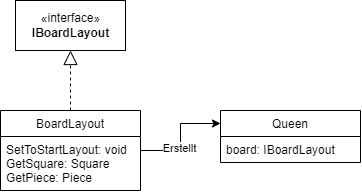
\includegraphics[width=9cm]{DependencyInjection.png}
		\caption{\label{pic:DependencyInjection}DependencyInjection in unserem Code}
	\end{center}
\end{figure}

\texttt{Boardlayout} implementiert die beiden Methoden \texttt{GetSquare} und \texttt{GetPiece} des Interfaces \texttt{IBoardLayout}. Wie der Namensgebung zu entnehmen ist, geben die Methoden ein \texttt{\href{https://github.com/schmida736/Chess-AdvancedSE/blob/main/Chess-AdvancedSE/Game\%20Elements/Pieces/Piece.cs}{Piece}} oder \texttt{\href{https://github.com/schmida736/Chess-AdvancedSE/blob/main/Chess-AdvancedSE/Game\%20Elements/Square.cs}{Square}} zurück. \\
Einzelne Figuren benötigen ein Objekt von \texttt{IBoardLayout}, welches im Konstruktor übergeben wird. Erzeugt nun das \href{https://github.com/schmida736/Chess-AdvancedSE/blob/main/Chess-AdvancedSE/Game\%20Elements/BoardLayout.cs}{BoardLayout} eine Dame, muss ein Verweis auf ein \texttt{IBoardLayout} übergeben werden. Eine Erzeugung sieht wie folgt aus:

\begin{lstlisting}[language=c, style=mStyle]
startLayout[0][0].Piece = new Queen(player.Color, this);
\end{lstlisting}

Der hier übergebene Parameter \texttt{this} verweist auf \texttt{\href{https://github.com/schmida736/Chess-AdvancedSE/blob/main/Chess-AdvancedSE/Game\%20Elements/BoardLayout.cs}{BoardLayout}}, welches das Interface \texttt{IBoardLayout} implementiert. Im Konstruktor von \texttt{\href{https://github.com/schmida736/Chess-AdvancedSE/blob/main/Chess-AdvancedSE/Game\%20Elements/Pieces/Queen.cs}{Queen}} muss dieses einer lokalen Variable von \texttt{IBoardLayout} zugeteilt werden. Da \texttt{\href{https://github.com/schmida736/Chess-AdvancedSE/blob/main/Chess-AdvancedSE/Game\%20Elements/Pieces/Queen.cs}{Queen}} nur das Interface \texttt{IBoardLayout}
und nicht das \texttt{\href{https://github.com/schmida736/Chess-AdvancedSE/blob/main/Chess-AdvancedSE/Game\%20Elements/BoardLayout.cs}{BoardLayout}} selbst kennt, kann sie auch nur auf die beiden Methoden des Interfaces zugreifen. Sie erhält damit lediglich eine Zugriffsmöglichkeit, bzw eine Schnittstelle, um die benötigten Ressourcen zu erhalten, ohne dabei eine Abhängigkeit auf die ganze Klasse zu haben. \texttt{\href{https://github.com/schmida736/Chess-AdvancedSE/blob/main/Chess-AdvancedSE/Game\%20Elements/Pieces/Queen.cs}{Queen}} ist dadurch auch von der Implementierung innerhalb von \texttt{\href{https://github.com/schmida736/Chess-AdvancedSE/blob/main/Chess-AdvancedSE/Game\%20Elements/BoardLayout.cs}{BoardLayout}} abgekapselt, da bei Änderung des Codes nur die Schnittstelle, gegeben durch das Interface, angepasst werden muss. Die Dame erhält ihre Informationen also nur aus der Schnittstelle und nicht direkt von \texttt{\href{https://github.com/schmida736/Chess-AdvancedSE/blob/main/Chess-AdvancedSE/Game\%20Elements/BoardLayout.cs}{BoardLayout}}.
\subsection{Command Pattern}
Das Command Pattern ist ein Verhaltensmuster, was bedeutet, dass es das Verhalten der Software beeinflusst. Die Hauptstruktur in bei diesem Muster ist der \texttt{Command}. Weitere sind der \texttt{Receiver}, der \texttt{Invoker} und der \texttt{Client}. Ein \texttt{Command} ist ein Objekt, welches einen Methodenaufruf an den \texttt{Reciever} einkapselt. Er enthält damit alle nötigen Informationen, die der \texttt{Invoker} braucht, um den Methodenaufruf auf \texttt{Receiver} ausführen zu können. \texttt{Client} ist der name des Moduls, das die anderen drei Objekte verwaltet.

Wir wollten das Command Pattern in unserem Programm umsetzen, da wir der Meinung waren, dass es sehr gut unsere Befehlsorientierte Architektur ergänzen könnte. So wäre \href{https://github.com/schmida736/Chess-AdvancedSE/blob/main/Chess-AdvancedSE/Game\%20Elements/Game.cs}{Game} der Client, welcher \texttt{Commands} von den Translators erhalten würde und diese dann an die \texttt{Invoker} \href{https://github.com/schmida736/Chess-AdvancedSE/blob/main/Chess-AdvancedSE/Game\%20Elements/Board.cs}{Board} oder Pieces verteilen würde.
Dies würde es uns erlauben, Befehle der GUI oder der Engine zu kapseln, in eine Queue abzulegen und nacheinander abzuarbeiten.

Während der Umsetzung des Musters haben wir aber gemerkt, dass diese nicht ohne grundlegende Veränderungen an unserer Architektur effizient umsetzbar ist. Das liegt daran, dass unsere \href{https://github.com/schmida736/Chess-AdvancedSE/blob/main/Chess-AdvancedSE/Game\%20Elements/Board.cs}{Board} und \href{https://github.com/schmida736/Chess-AdvancedSE/blob/main/Chess-AdvancedSE/Game\%20Elements/Pieces/Piece.cs}{Piece} Klassen schon zu sehr verknüpft sind, um diese unabhängig voneinander von \href{https://github.com/schmida736/Chess-AdvancedSE/blob/main/Chess-AdvancedSE/Game\%20Elements/Game.cs}{Game} aus anzusprechen.
Das zweite Problem ist, dass die Befehle aus der User-Interface-Schicht erst von Translators übersetzt werden müssen, bevor sie an \href{https://github.com/schmida736/Chess-AdvancedSE/blob/main/Chess-AdvancedSE/Game\%20Elements/Game.cs}{Game} weitergegeben werden können. Die Umsetzung des Musters wäre also möglich gewesen \\(Siehe git-branch \texttt{\href{https://github.com/schmida736/Chess-AdvancedSE/tree/command-pattern-integration}{command-pattern-integration}}), wäre aber auf das Verschicken von Befehlen zwischen den Translators und \texttt{\href{https://github.com/schmida736/Chess-AdvancedSE/blob/main/Chess-AdvancedSE/Game\%20Elements/Game.cs}{Game}} beschränkt gewesen. Dies ist zur Zeit über einen simplen Methodenaufruf geregelt, man würde also viel Komplexität für wenig Funktionalität erzeugen. Aus diesem Grund haben wir uns gegen die Implementierung entschieden, wie sie im git Branch zu sehen ist.
\newpage
\section{Fazit}
\label{sec:end}

Wir sind fest davon überzeugt, dass am Ende jedes Projekts die Entwickler mit dem Gedanken \textit{Im Nachhinein hätten wir vieles anders gemacht!} abschließen. Genau so geht es uns auch. Hätten wir beispielsweise von Anfang an für die Figuren eine wesentlich komplexere Klassenstruktur gewählt als \textit{alle erben von \href{https://github.com/schmida736/Chess-AdvancedSE/blob/main/Chess-AdvancedSE/Game\%20Elements/Pieces/Piece.cs}{Piece}!}, könnten Bauern leichter implementiert werden als es jetzt der Fall ist. Zudem hätte auf diese Weise wahrscheinlich auch die Wiederholung der Validierungsmethoden von Dame, Läufer und Turm verhindert werden können. \\
Ebenfalls wäre die Einbindung des Command-Pattern von Anfang an sinnvoller gewesen, da sich die Klassen an dieses Schema angepasst hätten anstatt im Nachhinein an vielen Stellen fummeln zu müssen damit die tolle Idee auch klappt. \\
Aber es gibt auch positive Rückmeldung an uns selbst: \textit{Auf die Clean Architecture sind wir stolz.} Es ist auch nicht ausgeschlossen dass wir eines Tages ein LED-Schach basteln / drucken und dafür einen großteil des Codes verwenden werden.\\
Wir sind froh, uns für die Implementierung von Schach entschieden zu haben. Nach Einsicht in den alten Code von vor drei Jahren gab es neben einigen Lachern auch das belohnende Gefühl wirklich was im Studium gelernt und die eigenen Programmierfähigkeiten gut ausgebaut zu haben. Wir freuen uns auf alles was noch kommt!


\end{onehalfspace}
\end{document}